\documentclass{ctexart}
\usepackage{geometry}
\usepackage{fancyhdr}
\usepackage{graphicx}
\usepackage{booktabs}
\usepackage{amsmath}
\usepackage{caption}
\usepackage{tikz}
\usepackage{array}
\xeCJKsetup{CJKmath=true} 
\usepackage{zhnumber} % change section number to chinese
\renewcommand\thesection{\zhnum{section}}
\renewcommand \thesubsection {\arabic{subsection}}
\CTEXsetup[format={\Large\bfseries}]{section}

\geometry{
    a4paper,
    left=3.18cm,
    right=3.18cm,
    top=3.04cm,
    bottom=3.04cm
}

\pagestyle{fancy}
\fancyhf{}
\renewcommand{\headrulewidth}{0.7pt} % 设置页眉横线粗细
\fancyhead[L]{\kaishu\large 大学物理实验报告} % 在左侧设置页眉文字
\fancyhead[R]{\kaishu\large 哈尔滨工业大学(深圳) } % 在右侧设置页眉文字
\fancyfoot[R]{\thepage} % 将页数放在右下角


\setlength\headwidth{\textwidth}

\begin{document}

\noindent
\textbf{
    \begin{tabular}{p{2.4cm}p{2.4cm}p{4cm}p{3.8cm}}
        班级 \hrulefill & 学号 \hrulefill & 姓名 \hrulefill & 教师签字 \hrulefill \\
    \end{tabular}\\
    \begin{tabular}{p{6cm}p{3.6cm}p{3.55cm}}
        \ 实验日期 \hrulefill & 预习成绩 \hrulefill & 总成绩 \hrulefill
    \end{tabular}\\
}
\rule[-10pt]{\textwidth}{0.7pt}

\begin{center}
    \Large \textbf{实验内容 \underline{液体黏度的测定}}
\end{center}

\section{预习内容}

实验指导书中提到,在本实验中,如果小钢球从蓖麻油液面处开始下落,初速度为零,最初是加速运动,随着速度的增大,其受到的黏滞力也将增大,因此该过程是一个加速度越来越小的加速运动。但是实际操作时,小钢球是从距离液面$h$高度开始下落的,请分析一下,小钢球进入蓖麻油之后,是做加速运动还是减速运动?设小钢球质量为$m$,直径为$d$,小球密度为$\rho$,蓖麻油密度为$\rho_0$,黏滞系数为$\eta    $,黏滞力由斯托克斯定律给出,无需作修正,忽略空气对小钢球的作用力。

\newpage
\section{实验现象及原始数据记录}

\begin{table}[h]
    \renewcommand\arraystretch{1.3}
    \centering
    \label{tab:m}
    \begin{tabular}{|m{2.8cm}<{\centering}|m{2.5cm}<{\centering}|m{2.5cm}<{\centering}|m{2.5cm}<{\centering}|}
        \multicolumn{4}{c}{螺旋测微器系统误差:$\rule{2.5cm}{0.3pt} \ mm $} \\
        \hline
        小钢球编号& 直径测量读数 $d(mm)$ & 蓖麻油温度$T(^\circ C)$ & 小钢球下落时间$t (s)$ \\
        \hline
        1 & & & \\
        \hline
        2 & & & \\
        \hline
        3 & & & \\
        \hline
        4 & & & \\
        \hline
        5 & & & \\
        \hline
        6 & & & \\
        \hline
    \end{tabular}
\end{table}

\begin{tikzpicture}[remember picture,overlay]
    \node[anchor=south east,inner sep=100pt] at (current page.south east) {
        \renewcommand{\arraystretch}{1.5} % 表格行高倍数
        \setlength{\tabcolsep}{18pt}    
    \begin{tabular}{|c|c|}
        \hline
        \LARGE  教师 & \LARGE  姓名 \\
        \hline
        \LARGE \kaishu 签字 &  \\
        \hline
        \end{tabular}
    };
\end{tikzpicture}

\newpage

\section{数据处理}

(利用测得的数据计算各温度下蓖麻油的黏度,绘出黏度-温度关系曲线,推导出$\eta$的相对不确定度公式,然后计算某个温度下$\eta$的不确定度,并完整表达测量结果,要有详细的计算过程,格式工整)

首先,$\eta$的相对不确定度公式的推导如下:


$$ S_{D} = \sqrt{\frac{\displaystyle\sum_{i=1}^{5}(d_i-\overline{d})^2}{n(n-1)}} = 0.002\  mm $$

$$ u_1 = \frac{\Delta_{\text{仪}}}{c} = 0.006 \  mm $$

$$ u_d = \sqrt{S_{D}^2 + u_1^2} = 0.006 \ mm $$

$$ u_t = \frac{\Delta_{\text{仪}}}{c} = 0.2\ s $$

推导总不确定度:

$$ \overline{\eta} = \frac{(\rho-\rho_0)gd^2t}{18L\cdot (1+2.4d/D)} $$

$$ E_\eta = \sqrt{\left(\frac{\partial \ln{n}}{\partial t}\right)^2u_t^2+\left(\frac{\partial \ln{n}}{\partial d}\right)^2u_d^2}= \sqrt{\frac{u_t^2}{t^2}+\left(\frac{2}{d} - \frac{2.4}{D+2.4d}\right)^2u_d^2} $$

$$ u_\eta = E_\eta \cdot \overline{\eta} $$

经过计算得到如下数据:(置信概率$P=68.3\%$)

\begin{table}[h]
    \renewcommand\arraystretch{1.3}
    \centering
    \begin{tabular}{|m{2.8cm}<{\centering}|m{2.5cm}<{\centering}|m{2.5cm}<{\centering}|m{2.5cm}<{\centering}|}
        \hline
        蓖麻油温度$T(^\circ C)$ & $液体粘度\eta \  (Pa\cdot s)$ & $u_\eta (Pa\cdot s)$ & 相对不确定度$E_\eta$ \ (\%) \\  
        \hline
        30 &0.488 & 0.0060 & 1.23\\
        \hline
        35 &0.317 & 0.0042 & 1.32\\
        \hline
        40 &0.236 & 0.0034 & 1.43\\
        \hline
        45 &0.176 & 0.0028 & 1.60\\
        \hline
        50 &0.130 & 0.0025 & 1.90\\
        \hline
        55 &0.099 & 0.0023 & 2.27\\
        \hline
    \end{tabular}
\end{table}

然后绘制了粘度-温度关系曲线如下:

\begin{figure}[h]
    \centering
    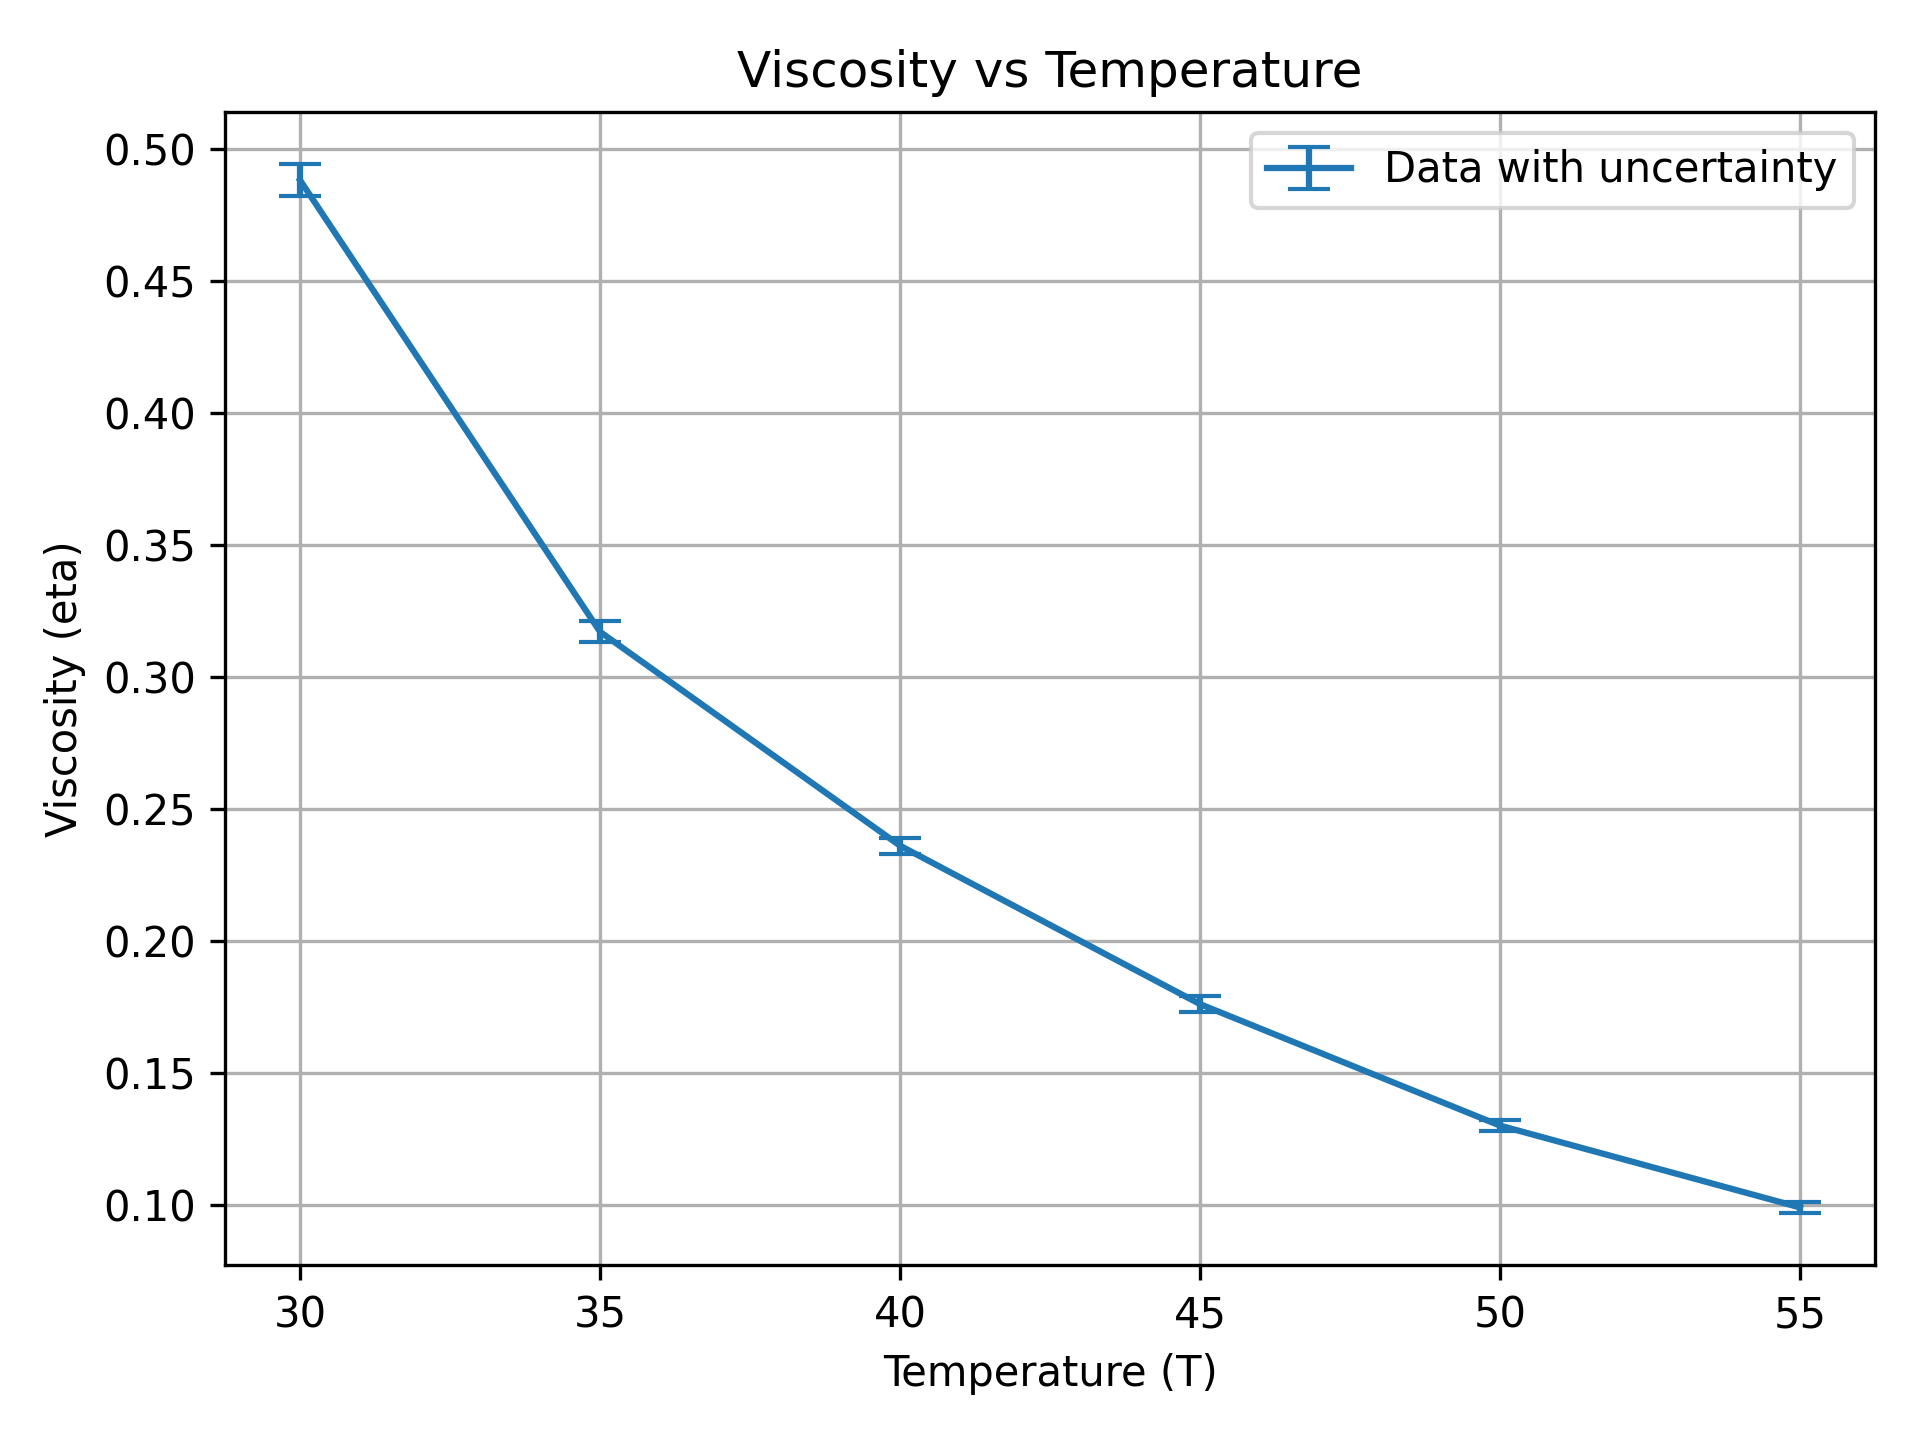
\includegraphics[width=0.75\textwidth]{vscsty_vs_tmprtr.png}
\end{figure}

\section{实验结论及现象分析}

计算结果显示,蓖麻油的黏度随着温度的升高而下降,这与实验现象相符合。在具体实验中,等待小球下落一段距离后才进行计时,在计时区间内下落观察到速度变化不大,近似为匀速运动。计算结果见上文。

\section{讨论题}

\subsection{讨论本实验中出现实验误差的原因。}

每一组实验中只计时一次,可能存在计时误差。其次,小球下落时无法完美处于中线下落,导致实验结果不准确。最后,实验中可能存在温度测量误差,导致实验结果不准确。

\subsection{请解释为什么液体的黏度是随着温度上升而下降。}

液体中的分子间距较小,彼此紧密排列。当温度升高时,分子的动能增加,促进了分子之间的流动,从而导致液体的黏度降低。

\subsection{如果小球在靠近玻璃管壁处下落,会对液体黏度的实验测量值有什么影响?}

实际观测到下落变慢,实验测量值会偏大;理论上:根据公式$$\eta = \frac{(\rho-\rho_0)gd^2t}{18L\cdot (1+2.4d/D)}$$相当于$D$偏大,$\eta$偏大。

\subsection{如果玻璃管是倾斜的,会对液体黏度的实验测量值有什么影响?}

实际上观察到所需时间变短;理论上同样根据上式,$L$偏小,$\eta$偏大。
\end{document}